\documentclass[12pt]{article}
\usepackage[spanish]{babel}
\usepackage{graphicx}
\usepackage{float}
\usepackage{listings}
\usepackage{xcolor}

\definecolor{codegreen}{rgb}{0,0.6,0}
\definecolor{codegray}{rgb}{0.5,0.5,0.5}
\definecolor{codepurple}{rgb}{0.58,0,0.82}
\definecolor{backcolour}{rgb}{0.95,0.95,0.92}


\lstdefinestyle{mystyle}{
	backgroundcolor=\color{backcolour},   
	commentstyle=\color{codegreen},
	keywordstyle=\color{magenta},
	numberstyle=\tiny\color{codegray},
	stringstyle=\color{codepurple},
	basicstyle=\ttfamily\footnotesize,
	breakatwhitespace=false,         
	breaklines=true,                 
	captionpos=b,                    
	keepspaces=true,                 
	numbers=left,                    
	numbersep=5pt,                  
	showspaces=false,                
	showstringspaces=false,
	showtabs=false,                  
	tabsize=2
}

\lstset{style=mystyle}

\title{Síntesis de redes activas \\ Filtro rechaza banda: Notch}

\author{Profesor Titular: Dr. Ing. Pablo Ferreyra \\  Profesor Adjunto: Ing. César Reale \\ Alumnos: Campos Mariano,	Enzo Verstraete}

\begin{document}
	\maketitle
	\newpage
	\section{Consigna}
	Diseñar un filtro NOTCH para ser utilizado en electrocardiograma (ECG), donde es fundamental
	filtrar la señal de 50Hz de la linea de tensión.
	
	Especificaciones: Fn=50Hz, Q=10, ancho de banda de caida 3db de 5Hz y sin ganancia.
	Ecuación del NOTCH:
	
	\begin{equation}
		H(jw)=\frac{An(s^2+wn^2)}{s^2+s\frac{wn}{Q}+wn}
	\end{equation}
	
	
	\section{Desarrollo}
	Un filtro Notch (o filtro de rechazo de banda) es un filtro diseñado para eliminar una frecuencia específica de una señal, dejando pasar el resto del espectro. Se caracteriza por tener una respuesta en frecuencia con una caída muy pronunciada (un notch o muesca) en torno a la frecuencia que desea atenuar.
	
	Para sintetizar el filtro, el primer paso es: en base a las especificaciones dadas,es obtener la función de transferencia global, para esto realizamos el siguiente análisis:
	
	\begin{lstlisting}
		%% Especificaciones del filtro
		fn = 50;          % Frecuencia central [Hz]
		Q = 10;           % Factor de calidad
		BW = 5;           % Ancho de banda 3dB [Hz]
		wo = 2 * pi * fn; % Frecuencia angular central [rad/s]
		bw_rad = 2 * pi * BW; % Ancho de banda en radianes/segundo
		
		%% Funcion de transferencia del filtro rechaza-banda
		% Coeficientes del denominador (forma estandar del filtro)
		den = [1, wo/Q, wo^2]; % Denominador: s^2 + (wo/Q)*s + wo^2
		% Coeficientes del numerador
		num = [1, 0, wo^2];    % Numerador: s^2 + wo^2 (estructura notch)
		
		% Crear la funcion de transferencia
		Filtro = tf(num, den)
	\end{lstlisting}
	
	La función de transferencia obtenida resulta:
	\begin{equation}
		H(s)=\frac{s^2+9.87e4}{s^2+31.42s+9.87e4}
	\end{equation}
	
	El segundo paso es descomponer esta función en la suma de dos bicuadráticas una para un filtro pasa alto y otra para el filtro pasa bajo:
	\begin{equation}
		H(s)=H_{LP}(s)+H_{HP}
	\end{equation}
	
	Donde:
	\begin{equation}
		H_{LP}(s)=\frac{wo^2}{s^2+s\frac{wo}{Q}+wo^2} , H_{HP}(s)=\frac{s^2}{s^2+s\frac{wo}{Q}+wo^2}
	\end{equation}
	
	\begin{lstlisting}
		%% Descomposicion manual en pasa-bajo y pasa-alto
		% Filtro pasa-bajo
		num_pb = [0, 0, wo^2]; % Numerador solo tiene la parte constante (s^0)
		den_pb = den;          % Denominador igual al filtro original
		PasaBajo = tf(num_pb, den_pb)
		
		% Filtro pasa-alto
		num_pa = [1, 0, 0];    % Numerador tiene solo la parte de s^2
		den_pa = den;          % Denominador igual al filtro original
		PasaAlto = tf(num_pa, den_pa)
		
		% Respuesta en frecuencia
		figure;
		bode(Filtro, PasaBajo, PasaAlto);
		legend('Rechaza Banda', 'Pasa-Bajo', 'Pasa-Alto');
		title('Respuesta en frecuencia: Rechaza Banda y secciones bicuadraticas');
	\end{lstlisting}
	
	Las dos funciones de transferencias resultan:
	\begin{equation}
		H_{LP}(s)=\frac{9.87e4}{s^2+31.42s+9.87e4}
	\end{equation}
	
	\begin{equation}
		H_{HP}(s)=\frac{s^2}{s^2+31.42s+9.87e4}
	\end{equation}
	
	Para verificar que el análisis es correcto realizamos la traza de Bode de las dos funciones de transferencias por separado (FPB+FPA) y la función de transferencia global
	\begin{figure}[h!]
		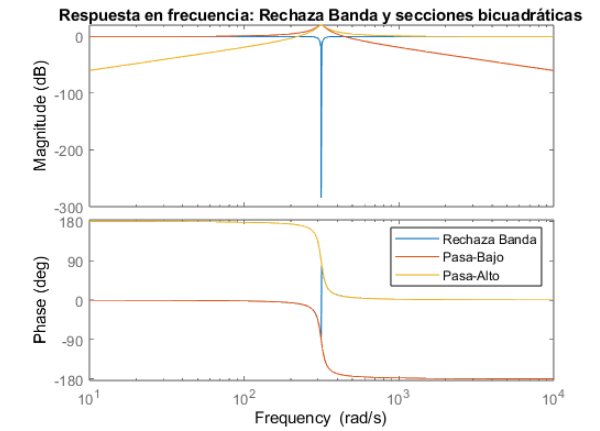
\includegraphics[width=1\linewidth]{Imagenes/Bode}
		\caption[Respuesta en frecuencia]{Respuesta en frecuencia}
		\label{fig:bode}
	\end{figure}
	
	\subsection{Filtro Sallen Key}
	Para implementar los filtros pasa bajo y pasa alto utilizamos un filtro Sallen-Key, es un circuito activo que utiliza un amplificador operacional (OpAmp) junto con resistencias y capacitores para implementar un filtro analógico de segundo orden. Es muy popular por su simplicidad y facilidad de ajuste de parámetros como la frecuencia de corte y ancho de banda.\newpage
	
	Análisis para la síntesis del filtro FPB:
	\begin{lstlisting}
	% Diseno del filtro pasa bajo Sallen Key
	syms C1 C2
	%Establecemos valores de resistencias
	R1=10e3
	R2=10e3
	
	%Planteamos las ecuaciones de wo y Q para calular C1 y C2
	equ1= wo == 1/sqrt(R1*R2*C1*C2);
	equ2= Q == sqrt(C1/C2)*sqrt(R1*R2)/(R1+R2);
	sol=solve([equ1, equ2],[C1 C2]);
	C1sol=double(sol.C1(2))
	C2sol=double(sol.C2(2))
	\end{lstlisting} 
	
	Valores de resistencias y capacitores: $R1=R2=10[Kohm]$, $C1=6.36[uF]$, $C2=15.9[nF]$
	Se implementa el filtro con un amplificador operacional LM324 y los valores de resistencias/capacidades obtenidas, ademas simulamos la respuesta en modulo y fase del filtro para verificar su correcto funcionamiento:
	\begin{figure}[h!]
		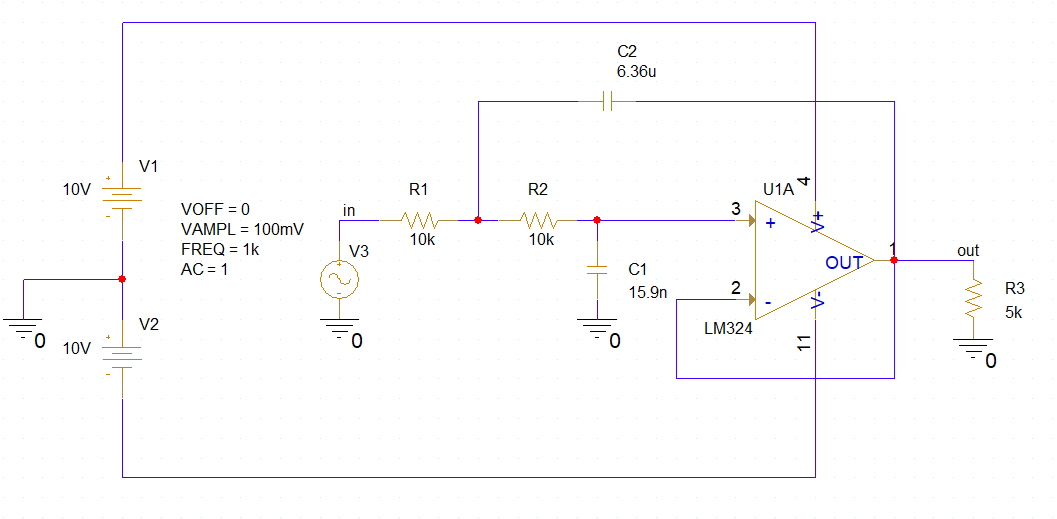
\includegraphics[width=1\linewidth]{Imagenes/FPB}
		\caption[Filtro pasa bajo Sallen Key]{Filtro pasa bajo Sallen Key}
		\label{fig:fpb}
	\end{figure}
	
	\begin{figure}
		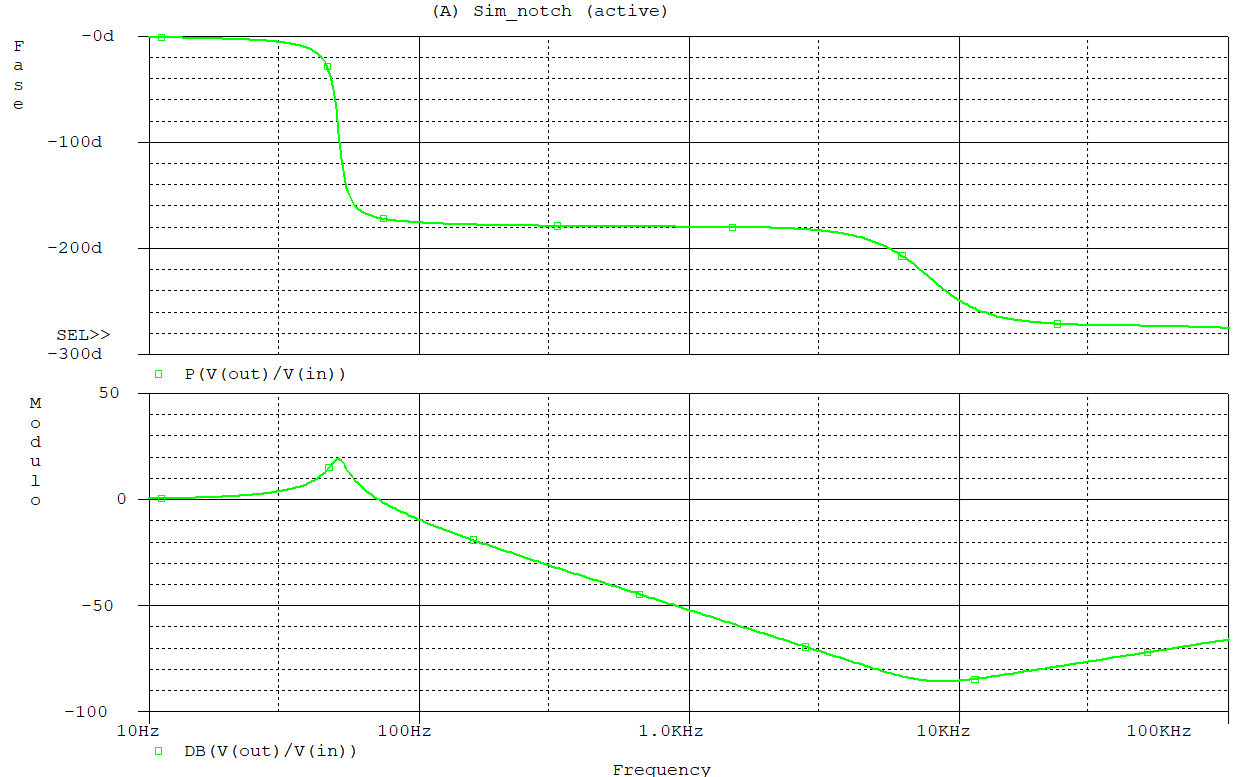
\includegraphics[width=1\linewidth]{Imagenes/Bode_FPB}
		\caption[Bode FPB]{Bode FPB}
		\label{fig:bodefpb}
	\end{figure}\newpage
	
	Análisis para la síntesis del filtro FPA:
	\begin{lstlisting}
	% Diseno del filtro pasa alto Sallen Key
	syms R1 R2
	%Establecemos valores de capacidad
	C1=100e-9
	C2=100e-9
	k=1 %retroalimentacion unitaria
	
	%Planteamos las ecuaciones de wo y Q para calular R1 y R2
	equ1= wo == 1/sqrt(R1*R2*C1*C2);
	equ2= Q == 1/(sqrt(R1/R2)*((C1+C2)/(sqrt(C1*C2)))+(1-k)*sqrt((R2*C2)/(R1*C1)));
	sol=solve([equ1, equ2],[R1 R2]);
	R1sol=double(sol.R1(2))
	R2sol=double(sol.R2(2))	
	\end{lstlisting}
	
	Valores de resistencias y capacitores: $C1=C2=100[nF]$, $R1=1.59[Kohm]$, $R2=636[Kohm]$ \newpage
	\begin{figure}[h!]
		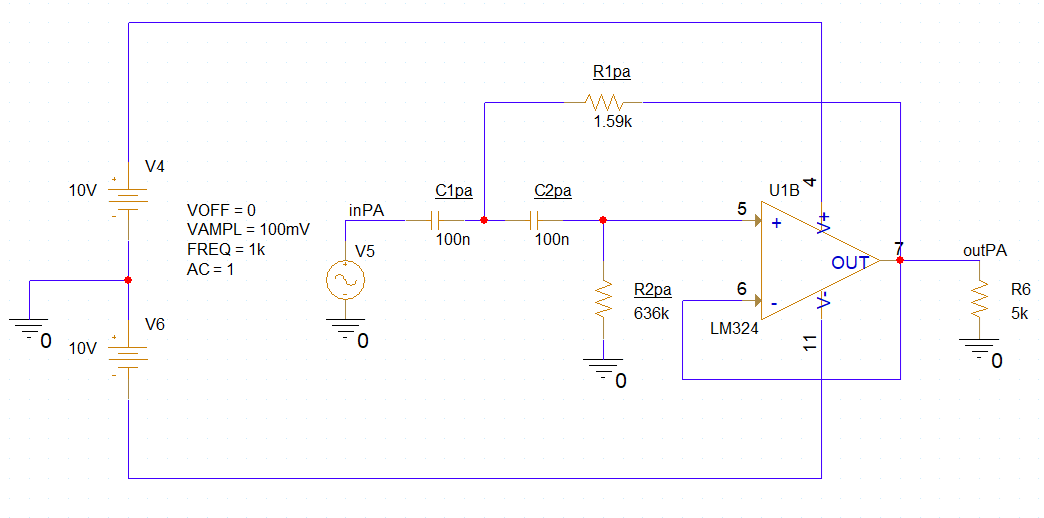
\includegraphics[width=1\linewidth]{Imagenes/FPA}
		\caption[Filtro pasa alto Sallen Key]{Filtro pasa alto Sallen Key}
		\label{fig:fpa}
	\end{figure}
	
	\begin{figure}[h!]
		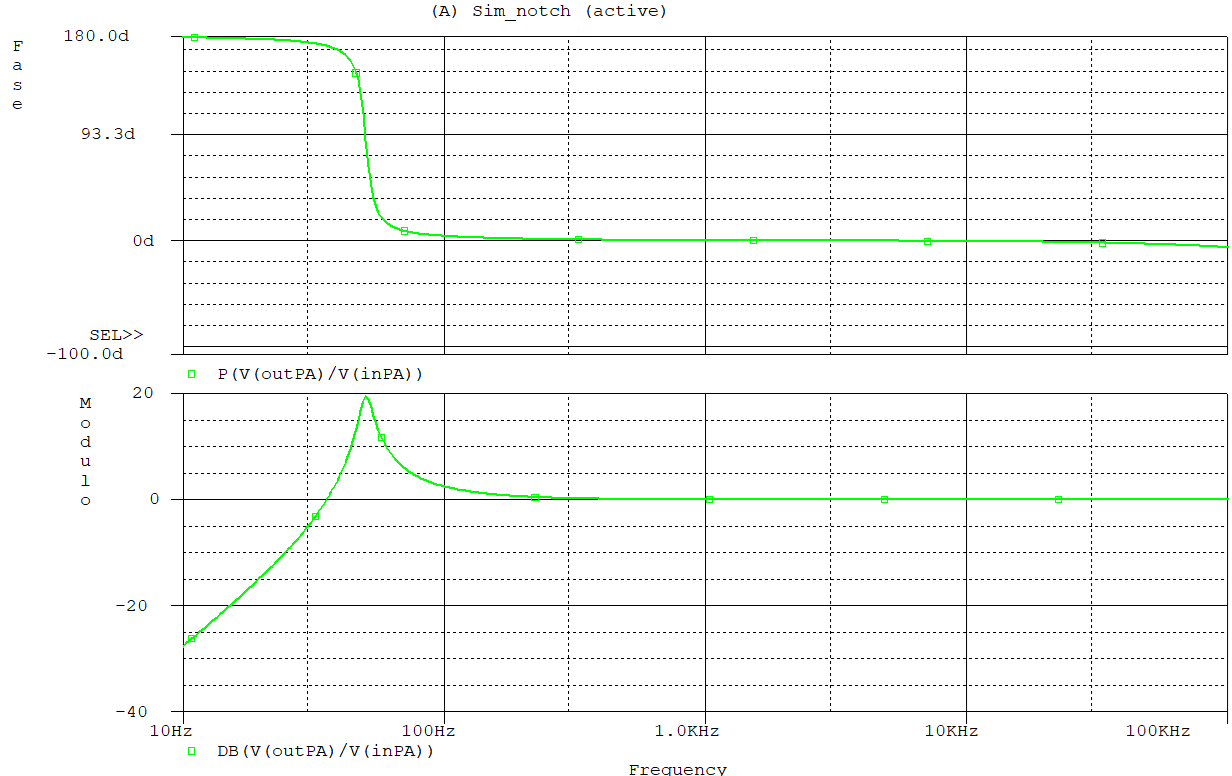
\includegraphics[width=1\linewidth]{Imagenes/Bode_FPA}
		\caption[Bode FPA]{Bode FPA}
		\label{fig:bodefpa}
	\end{figure}
	
	Una vez verificado que las funciones de transferencias están correctamente sintetizadas el siguiente paso es obtener la función de transferencia global que corresponde al filtro rechaza banda, esta resulta de la suma de las funciones individuales, para esto utilizamos un tercer amplificador operacional que sume las dos salidas.El circuito completo resulta:
	\begin{figure}[h!]
		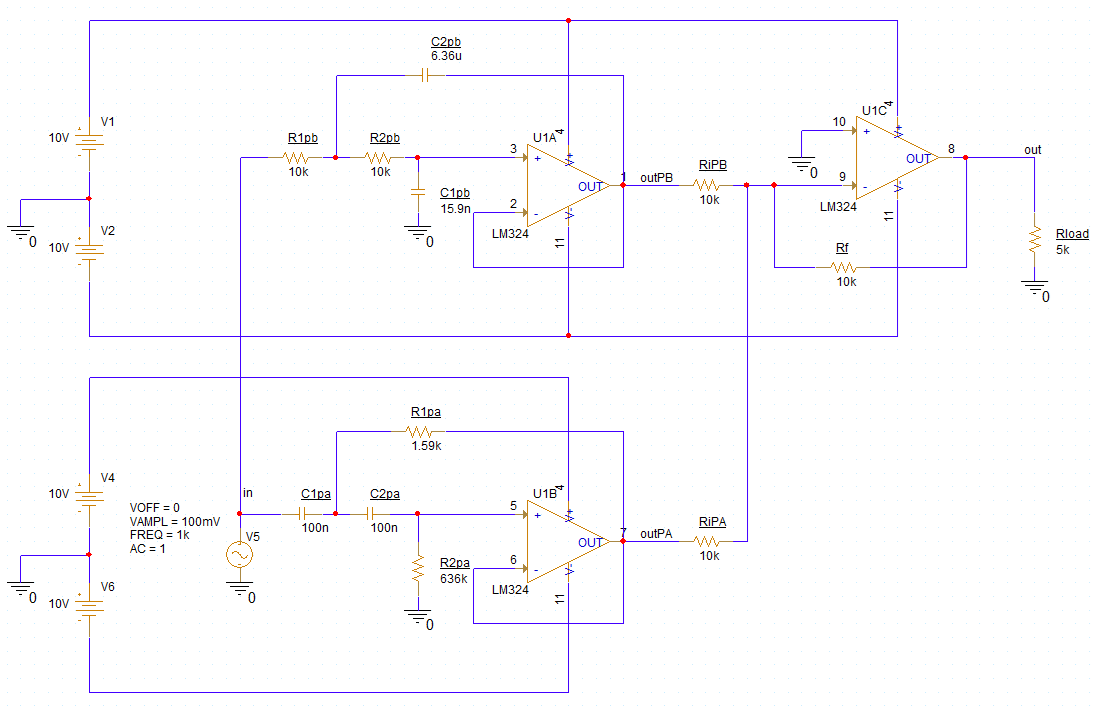
\includegraphics[width=1\linewidth]{Imagenes/Circuito_Completo}
		\caption[Circuito completo]{Circuito completo}
		\label{fig:circuitocompleto}
	\end{figure}
	
	Por ultimo para verificar la respuesta ideal a la que nos queríamos aproximar (Figura 1), realizamos la repuesta en frecuencia del filtro, de la figura 7 verificamos que la síntesis se a realizado con éxito.
	\begin{figure}[h!]
		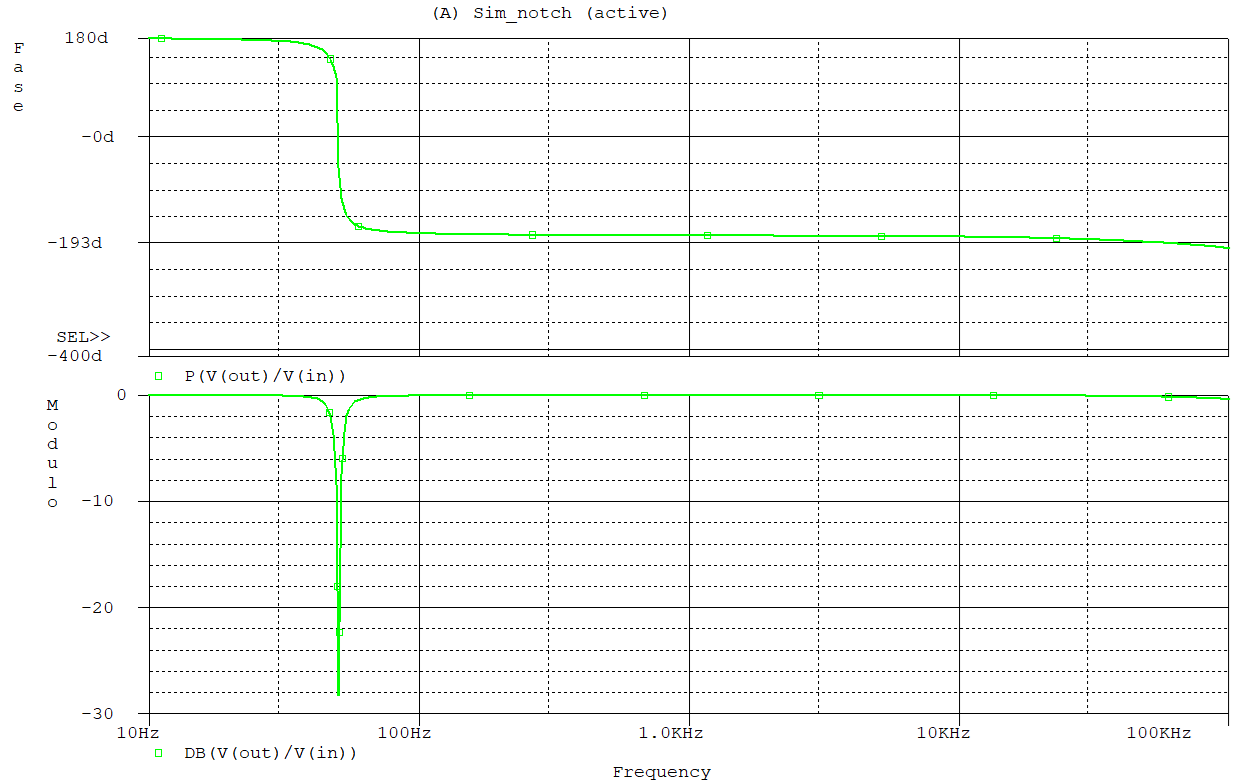
\includegraphics[width=1\linewidth]{Imagenes/Bode_Notch}
		\caption[Respuesta en frecuencia del filtro Notch]{Respuesta en frecuencia del filtro Notch}
		\label{fig:bodenotch}
	\end{figure}
	
	\subsection{Análisis de Montecarlo}
	Por ultimo realizamos un análisis de Montecarlo, no interesa saber que tan sensible resulta el filtro a las distintas tolerancias de los componentes, para eso le aplicamos a todos los componentes una tolerancia del diez por ciento, y corremos 50 simulaciones con una distribución gaussiana, el resultado es el siguiente:
	
	Se puede concluir que el filtro es muy sensible a los valores de las resistencias y capacidades, ya que una pequeña variación es estas producen un gran cambio en las magnitudes tanto del modulo como de la fase, se recomienda utilizar componentes con tolerancias del 1 por ciento.
	\begin{figure}
		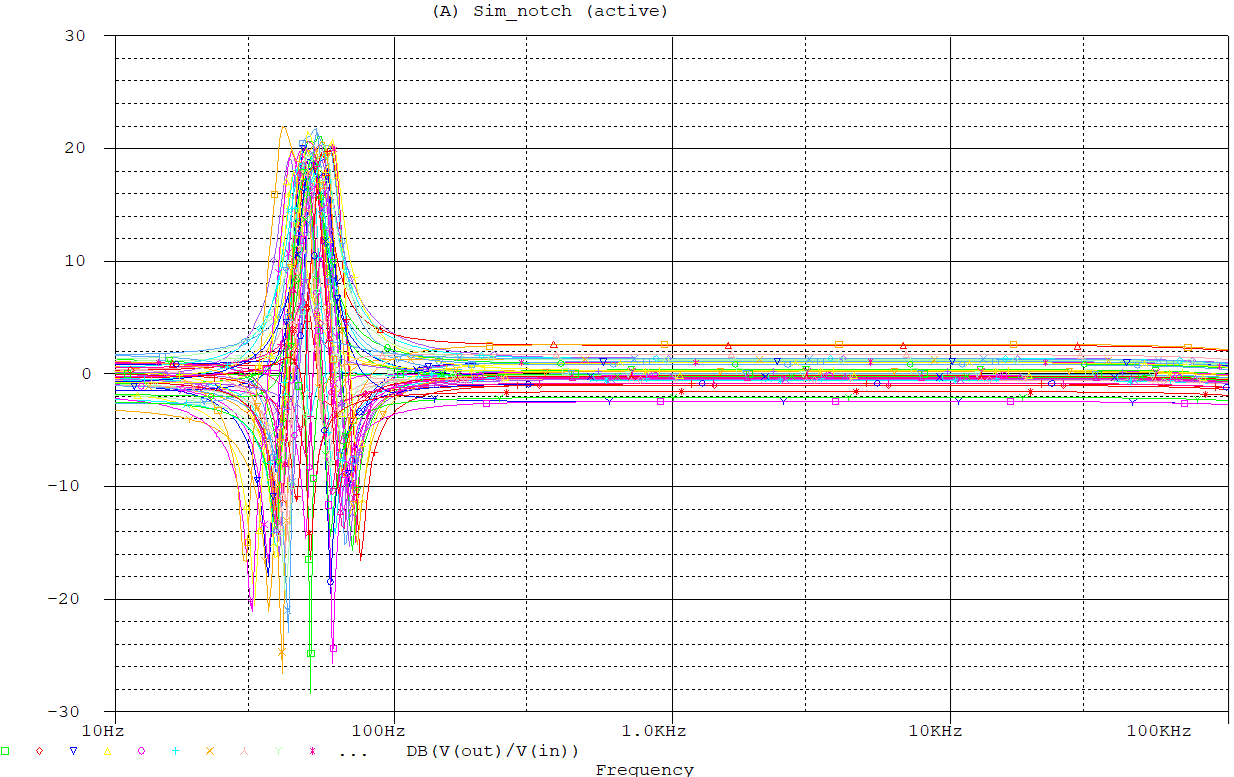
\includegraphics[width=1\linewidth]{Imagenes/montecarlo_modulo}
		\caption[Analsis de montecarlo para el modulo]{Analsis de montecarlo para el modulo}
		\label{fig:montecarlomodulo}
	\end{figure}
	
	\begin{figure}
		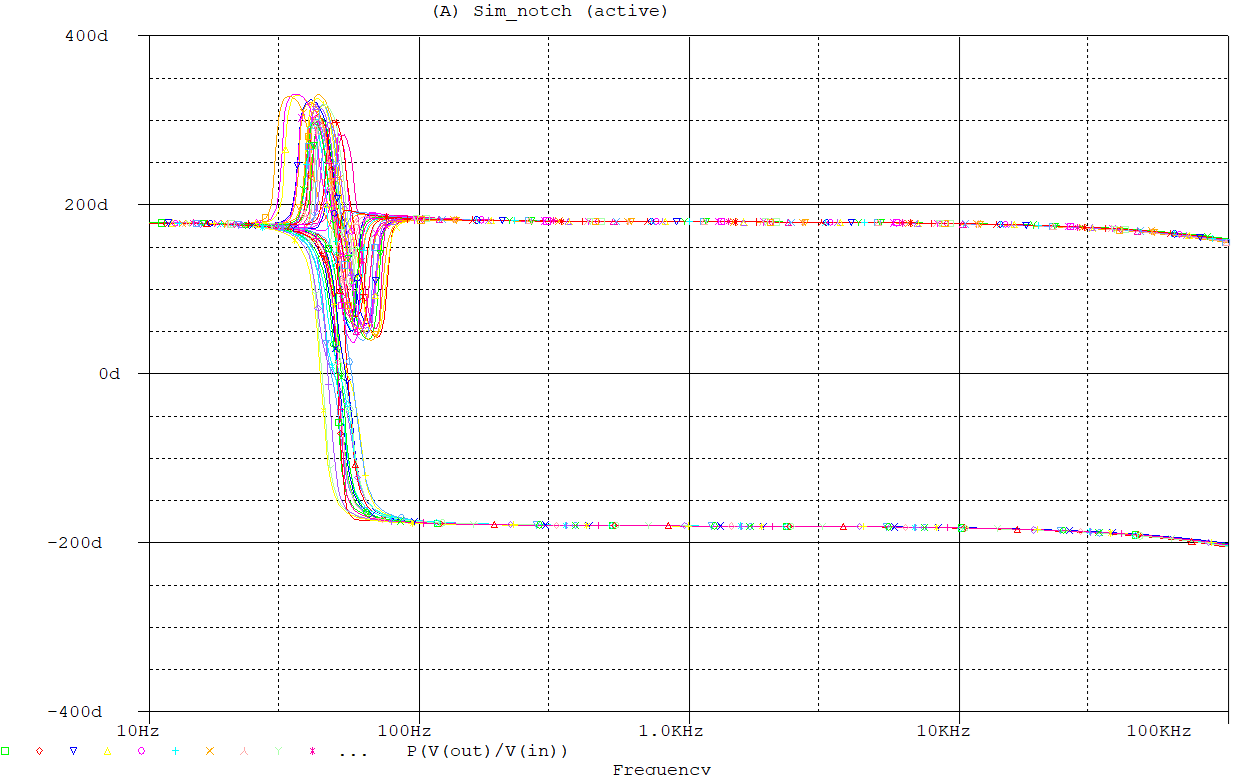
\includegraphics[width=1\linewidth]{Imagenes/montecarlo_fase}
		\caption[Análisis Montecarlo para la fase]{Análisis Montecarlo para la fase}
		\label{fig:montecarlofase}
	\end{figure}\newpage
	
	En las peores condiciones podemos ver que el filtro rechaza banda pasa a amplificar la señal que se desea suprimir resultando en un problema muy grave, esto es porque una pequeña variación en la frecuencia de corte hace que la FdT resultante se amplifique en esa banda.
	\begin{figure}
		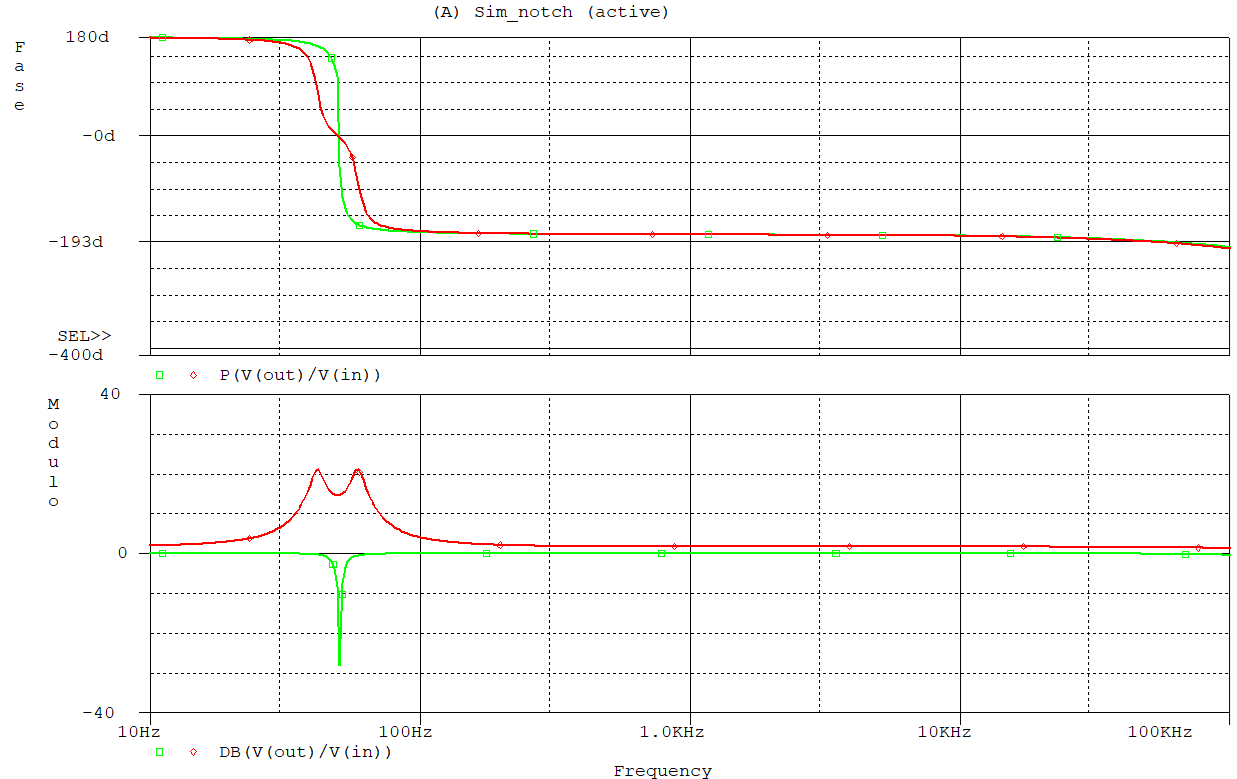
\includegraphics[width=1\linewidth]{Imagenes/peor_condicion}
		\caption[Respuesta del circuito en la peor condición (rojo)]{Respuesta del circuito en la peor condición (rojo)}
		\label{fig:peorcondicion}
	\end{figure}
	
	
	
	
	
\end{document}
}